\documentclass[english,compress]{beamer}

\usepackage{amsmath}
\usepackage{amssymb}
\usepackage[english]{babel}
\usepackage{tikz}
\usepackage{mathtools}
\usepackage{graphicx}
\usepackage{subfigure}
\usepackage{beamerthemeMadrid}
\usepackage{default}
\usepackage[square,numbers]{natbib}

\renewcommand{\bibsection}{\subsection*{\bibname}}

%Adding more spacing in itemize
\newlength{\wideitemsep}
\setlength{\wideitemsep}{\itemsep}
\addtolength{\wideitemsep}{5pt}
\let\olditem\item
\renewcommand{\item}{\setlength{\itemsep}{\wideitemsep}\olditem}

% Beamer options
\setbeamertemplate{section page}
{
	\begin{centering}
	\begin{beamercolorbox}[sep=12pt,center]{part title}
	\usebeamerfont{section title}\insertsection\par
	\end{beamercolorbox}
	\end{centering}
}
\beamertemplatenavigationsymbolsempty
\AtBeginSection{\frame{\sectionpage}}
\addtobeamertemplate{navigation symbols}{}{%
    \usebeamerfont{footline}%
    \usebeamercolor[fg]{footline}%
    \hspace{1em}%
    \insertframenumber/\inserttotalframenumber
}
\useoutertheme{split}
\useinnertheme{rectangles}
\usecolortheme{uiuc}
\logo{
\includegraphics[height=0.5cm]{uiuclogo.pdf}}
\expandafter\def\expandafter\insertshorttitle\expandafter{%
    \insertshorttitle\hfill\insertframenumber\,/\,\inserttotalframenumber}

\newcommand{\norm}[1]{\left\lVert #1 \right\rVert}
\newcommand{\abs}[1]{|#1|}
\newcommand{\vect}[1]{\boldsymbol{\mathbf{#1}}}
\newcommand{\ceil}[1]{\left \lceil #1 \right \rceil }
\newcommand{\floor}[1]{\left \lfloor #1 \right \rfloor }
\newcommand{\q}{ {\bf q} }

\title{Parallel Belief Propagation}
\subtitle{Image Super-Resolution}
\date{December 9, 2014}
\author{Nate Bowman, Erin Carrier, Anirudh Jayakumar, Ralf Gunter}

\begin{document}
\nocite{*}

\frame{\titlepage}
\frame{\frametitle{Table of contents}\tableofcontents}

\section{Introduction}
\frame{\frametitle{Overview}
	\begin{itemize}
	\item Algorithm designed to improve resolution of images
	\item Pixel-based images used as input
	\item Standard algorithms produce blurry images
	\item Large images created from small images
	\end{itemize}
}

\section{Image Super-Resolution}
\subsection{Basics}
\frame{\frametitle{Properties and Goals of the Algorithm}
	\begin{itemize}
	\item Uses machine learning
	\item Creates plausible high-frequency details
	\item Estimates details unobtainable by simple interpolation
	\end{itemize}
}

\subsection{Training}
\frame{\frametitle{Training}
	\begin{itemize}
	\item Learns fine details corresponding to image regions seen at low frequency
	\item Generates low-frequency patches: \\
		\framebox{image} $\xrightarrow{blur+subsample}$
		\framebox{} $\xrightarrow[highpass]{interpolate}$ 
		\framebox{low} $\xrightarrow{chunk}$ \framebox{low patches}
	\item Creates high-frequency patches: \\
		\framebox{image} $\xrightarrow{highpass\;filter}$
		\framebox{high}  $\xrightarrow{chunk}$ \framebox{high patches}
	\item Stores association: \\
		\begin{tabular}{| c | c |}
			\hline
			low patch &  high patch \\
			\hline
		\end{tabular}
	\end{itemize}
}
\frame{\frametitle{Training Optimizations}
	\begin{itemize}
	\item Keeps only highest frequencies of low-frequency images
	\item Locally normalizes contrast to reduce duplicates
	\end{itemize}
}

\subsection{Algorithm}
\frame{\frametitle{Overall Algorithm}
	\begin{itemize}
	\item Use cubic-spline interpolation to upsample input image
	\item Contrast normalize upsampled image and break into patches
	\item Solve for maximum probability high-frequency patch set in Markov network
	\item Contrast denormalize high-frequency patches
	\item Add resulting high-frequency patches to upsampled image
	\end{itemize}
}
\frame{\frametitle{Markov Network}
	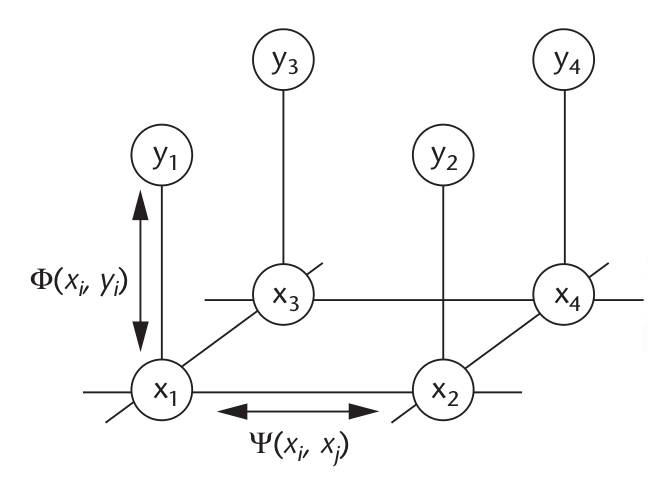
\includegraphics[width=.8\linewidth]{images/markov}
}
\frame{\frametitle{Markov Network}
	\begin{itemize}
	\item $x_i$: Unknown high-frequency patch. Modeled as a random variable. \\
		$x_i = \left\{\fbox{Patch}, \fbox{Patch}, \hdots, \fbox{Patch}\right\}$
	\item $y_i$: Observed (upsampled input) patch
	\item $P(x|y) = \frac{1}{Z}\prod_{(ij)}\psi_{ij}(x_i, x_j)\prod_i\phi_i(x_i, y_i)$
	\item $d_{ij}(x_i, x_j)$: sum of squared differences in overlap region
	\item $\psi_{ij}(x_i, x_j) = \exp(-\frac{d_{ij}(x_i, x_j)}{2\sigma^2})$
	\item Similar formula for $\phi_i(x_i, y_i)$
	\end{itemize}
}
\frame{\frametitle{Belief Propagation}
	\begin{itemize}
	\item Fast iterative algorithm
	\item Message: $m_{ij}(x_j)= \frac{1}{Z} \sum_{x_i}\psi_{ij}(x_i, x_j)\prod_{k \ne j}m_{ki}(x_i)\phi_i(x_i,y_i)$
	\item Belief: $b_i(x_i)=\prod_km_{ki}(x_i)\phi_i(x_i,y_i)$
	\item Iterate until convergence of beliefs
	\item Choose patches with the highest belief
	\end{itemize}
}
\frame{\frametitle{Results}
	\begin{itemize}
	\item Leads to an image that:
		\begin{itemize}
		\item is a good match for each patch
		\item maintains overall look of original image
		\item contains high-resolution features
		\end{itemize}
	\item Can add a weighting factor to favor $\phi$ or $\psi$
	\item Uses a generic training set
	\end{itemize}
}

\subsection{Example Results}
\frame{\frametitle{Example Image}
	\centering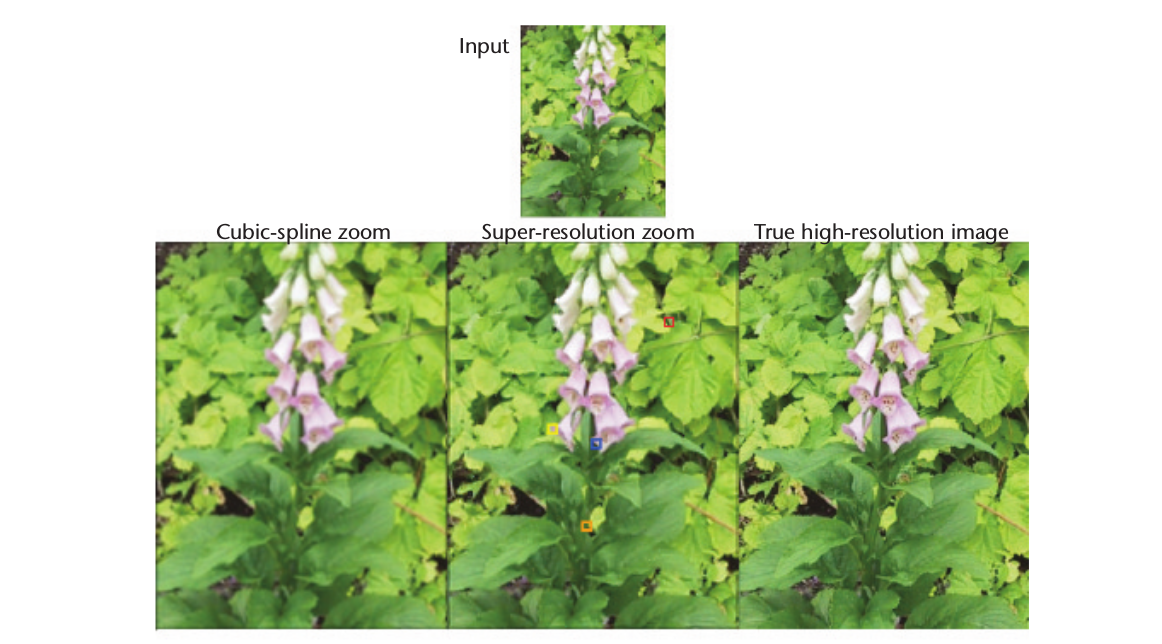
\includegraphics[scale=.25]{images/flower}
}
\frame{\frametitle{Example Image}
	\begin{center}
	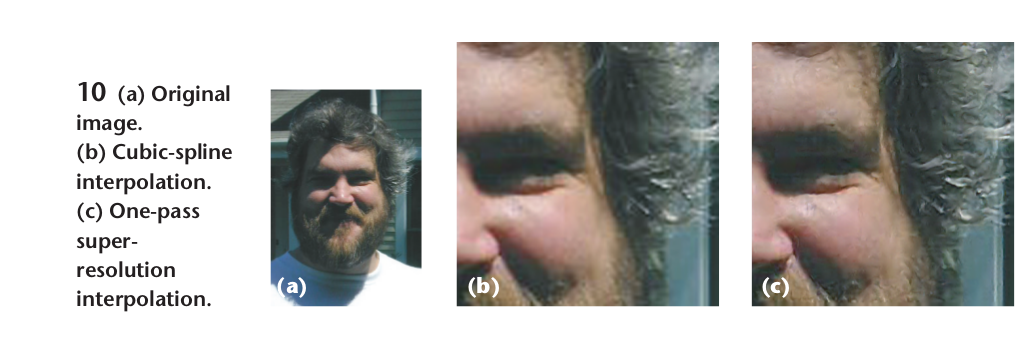
\includegraphics[scale=.3]{images/beard}
	\end{center}
}

\section{Our Implementation}
\subsection{Overview}
\frame{\frametitle{Phases}
	\begin{itemize}
	\item Preprocessing
	\item Parallel Belief Propagation
	\item Postprocessing
	\end{itemize}
}
\subsection{Preprocessing}
\frame{\frametitle{Preprocessing}
	\begin{itemize}
	\item Implemented in Python
	\item Builds training set patch pairs
		\begin{itemize}
		\item Blur, subsample, cubic-spline interpolate, high-pass filter, chunk, contrast normalize $\rightarrow$ low-frequency patches
		\item High-pass filter, chunk, contrast normalize $\rightarrow$ high-frequency patches
		\item Outputs patch pairs to file
		\end{itemize}
	\item Build input image patches
		\begin{itemize}
		\item Upsample, high-pass filter, chunk, contrast normalize
		\item Outputs input patches to file
		\end{itemize}
	\end{itemize}
}
\subsection{Belief Propagation}
\frame{\frametitle{Design Decisions:  Components}
	\begin{itemize}
	\item 2D chare array for storing patches
	\item One patch per chare
	\item Utilized node groups
		\begin{itemize}
		\item One copy of the database per node
		\end{itemize}
	\item Integrated LSH (Locality sensitive hashing) search for candidates
	\end{itemize}
}
\frame{\frametitle{Design Decisions:  Distributed DB}
	\begin{itemize}
	\item DB split across the nodes
	\item Requests sent to node group to find candidates
	\item Callback invoked on chare array element with selected candidate IDs
	\item Each chare finds best 16 candidates
	\end{itemize}
}
\frame{\frametitle{Parallel Program Flow}
	\begin{center}
	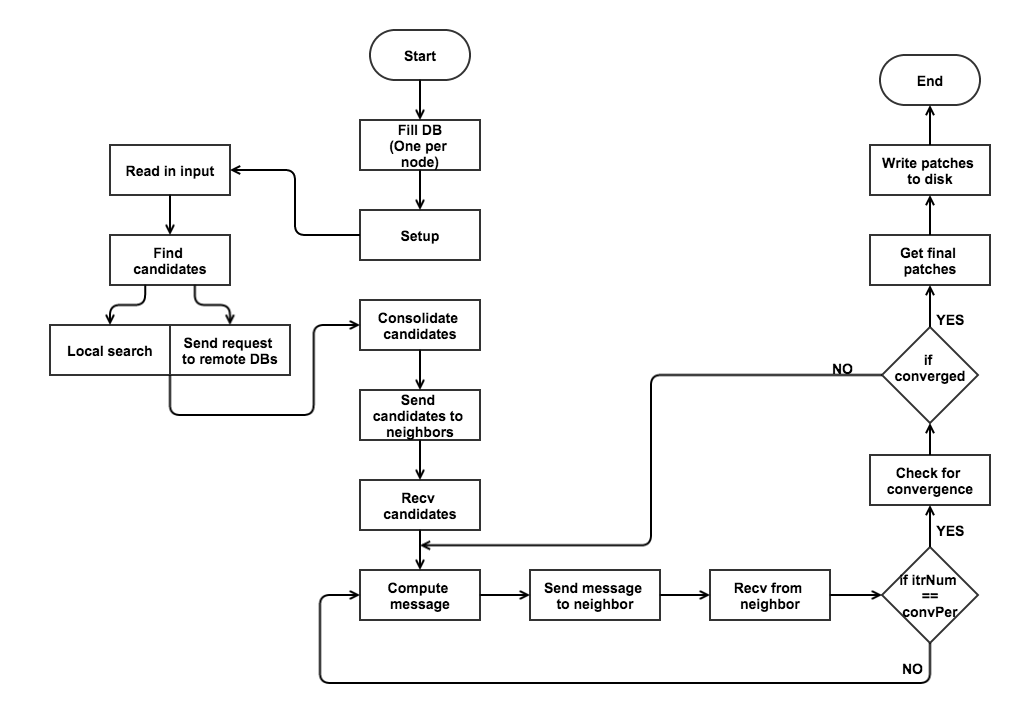
\includegraphics[scale=.3]{images/flow}
	\end{center}
}
\subsection{Postprocessing}
\frame{\frametitle{Postprocessing}
	\begin{itemize}
	\item Reads in chosen high-frequency patches
	\item Contrast denormalizes patches
	\item Adds patches to upsampled input to create high-resolution image
	\end{itemize}
}

\frame{\frametitle{References}
	\bibliographystyle{plainnat}
	\bibliography{bibentries}
}
\end{document}
